% Figure 2: Roofline Model — Prefill vs Decode
% Standalone compilable: pdflatex fig2_roofline.tex
\documentclass[border=5pt]{standalone}
\usepackage{tikz}
\usepackage{pgfplots}
\pgfplotsset{compat=1.18}

\begin{document}
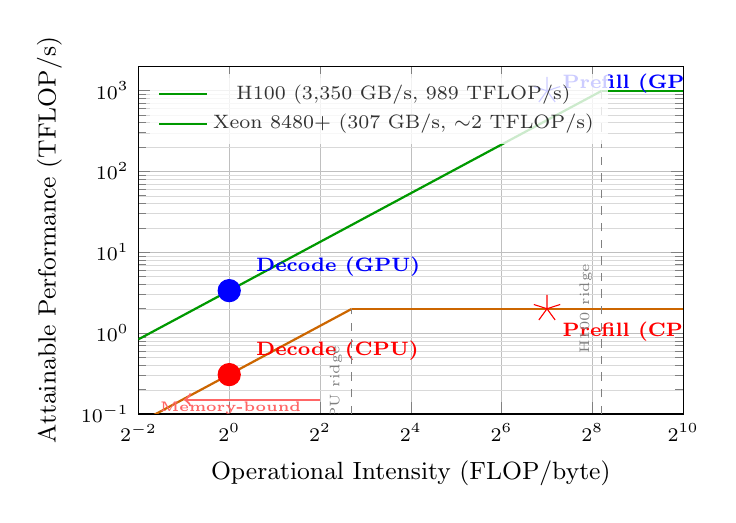
\begin{tikzpicture}
\begin{axis}[
    width=8.5cm,
    height=6cm,
    xmode=log,
    ymode=log,
    log basis x=2,
    log basis y=10,
    xlabel={Operational Intensity (FLOP/byte)},
    ylabel={Attainable Performance (TFLOP/s)},
    xmin=0.25, xmax=1024,
    ymin=0.1, ymax=2000,
    grid=both,
    grid style={line width=0.1pt, draw=gray!30},
    major grid style={line width=0.2pt, draw=gray!50},
    legend style={at={(0.02,0.98)}, anchor=north west, font=\scriptsize, draw=none, fill=white, fill opacity=0.8},
    tick label style={font=\scriptsize},
    label style={font=\small},
  ]

  % H100 Memory BW ceiling: 3.35 TB/s = 3350 GB/s
  % Ridge point: 989 / 3.35 = 295 FLOP/byte
  % H100 Compute ceiling: 989 TFLOP/s

  % H100 Roofline - memory slope
  \addplot[thick, color=green!60!black, domain=0.25:295] {3.35 * x};
  % H100 Roofline - compute ceiling
  \addplot[thick, color=green!60!black, domain=295:1024] {989};
  \addlegendentry{H100 (3,350 GB/s, 989 TFLOP/s)}

  % CPU Memory BW ceiling: 307 GB/s = 0.307 TB/s
  % CPU Compute ceiling: ~2 TFLOP/s (BF16 AMX rough estimate)
  % Ridge point: 2 / 0.307 = 6.5 FLOP/byte

  % CPU Roofline - memory slope
  \addplot[thick, color=orange!80!black, domain=0.25:6.5] {0.307 * x};
  % CPU Roofline - compute ceiling
  \addplot[thick, color=orange!80!black, domain=6.5:1024] {2.0};
  \addlegendentry{Xeon 8480+ (307 GB/s, $\sim$2 TFLOP/s)}

  % Decode point (OI = 1 for BF16)
  \addplot[only marks, mark=*, mark size=4pt, color=red, fill=red]
    coordinates {(1, 0.307)};
  \node[anchor=south west, font=\scriptsize\bfseries, color=red] at (axis cs:1.3, 0.35) {Decode (CPU)};

  \addplot[only marks, mark=*, mark size=4pt, color=blue, fill=blue]
    coordinates {(1, 3.35)};
  \node[anchor=south west, font=\scriptsize\bfseries, color=blue] at (axis cs:1.3, 3.8) {Decode (GPU)};

  % Prefill point (OI ~ 100-200 for long sequences)
  \addplot[only marks, mark=star, mark size=5pt, color=blue, fill=blue]
    coordinates {(128, 989)};
  \node[anchor=south west, font=\scriptsize\bfseries, color=blue] at (axis cs:140, 700) {Prefill (GPU)};

  \addplot[only marks, mark=star, mark size=5pt, color=red, fill=red]
    coordinates {(128, 2.0)};
  \node[anchor=north west, font=\scriptsize\bfseries, color=red] at (axis cs:140, 1.8) {Prefill (CPU)};

  % Ridge point annotations
  \draw[dashed, thin, gray] (axis cs:295,0.1) -- (axis cs:295,989);
  \node[font=\tiny, color=gray, anchor=south, rotate=90] at (axis cs:295, 2) {H100 ridge};

  \draw[dashed, thin, gray] (axis cs:6.5,0.1) -- (axis cs:6.5,2.0);
  \node[font=\tiny, color=gray, anchor=south, rotate=90] at (axis cs:6.5, 0.2) {CPU ridge};

  % Memory-bound region annotation
  \draw[<-, thick, color=red!60] (axis cs:0.5, 0.15) -- (axis cs:4, 0.15);
  \node[font=\tiny\bfseries, color=red!60, anchor=west] at (axis cs:0.3, 0.12) {Memory-bound};

\end{axis}
\end{tikzpicture}
\end{document}
